\documentclass[journal]{IEEEtran}
\usepackage{subcaption} 
\usepackage{color}
\usepackage{graphicx}
\usepackage{amsfonts}
\usepackage{amssymb}
\usepackage{siunitx}
\usepackage{url}
\usepackage{comment}
\usepackage{multirow}
\newcolumntype{N}{>{\centering\arraybackslash}m{.45in}}
\usepackage{colortbl,multirow,hhline,makecell}
\usepackage[table]{xcolor}
\newcommand{\abv}[1]{{\color{red}{[#1]}}}
\newcommand{\rever}{\textcolor{blue}}
%\newcommand{\rever}[1]{{\color{blue}{[#1]}}}
\newcommand{\refazer}[1]{{\color{red}{[#1]}}}
\newcommand{\gn}[1]{{\color{red}{[#1]}}}

\usepackage{placeins}
\usepackage{float}
\usepackage[english,brazilian]{babel}
%\usepackage[english]{babel}
\usepackage[utf8]{inputenc}
\usepackage[T1]{fontenc}
\usepackage{comment}
\usepackage{xcolor}
% correct bad hyphenation here
\hyphenation{op-tical net-works semi-conduc-tor}
\usepackage{cite}

\begin{document}
\title{Cryptography Algorithms in Wearable %Device
Communication: An Empirical Analysis}

%\author{{\bf Kristtopher~Kayo~Coelho}, {\bf Danilo~Damião}%~\IEEEmembership{Members,~IEEE,      	{\bf Alex~Borges},\\ %~\IEEEmembership{Fellow,~OSA,    {\bf Michele~Nogueira}, %~\IEEEmembership{Senior Member,~IEEE,}    {\bf Jos\'e Augusto M. Nacif},   {\bf Guevara Noubir}%,~\IEEEmembership{Life~Fellow,~IEEE}% <-this % stops a space
%\thanks{K. Coelho, D. Damião and J. Nacif is with the Science and Technology Institute, Federal University of Viçosa, Brazil} 

%\thanks{A. Borges is with the Department of Computer Science, Federal University of Juiz de Fora, Brazil.}% <-this % stops a space
%\thanks{M. Nogueira is with the Departmentof Computer Science, Federal University of Paran\'a, Brazil.}
%\thanks{G. Noubir is with the Department of Computer Science, Northeastern University, USA.
%}% <-this % stops a space
%\thanks{Manuscript received XX XX, 2018; revised August 26, 2015.}
%\vspace{-1.2cm}}

\author{%\vspace{-0.2cm}
{\bf Author 1}, {\bf Author 2}, %~\IEEEmembership{Members,~IEEE,
{\bf Author 3}, %~\IEEEmembership{Fellow,~OSA,   
{\bf Author 4}, %~\IEEEmembership{Senior Member,~IEEE,}    
{\bf Author 5}, {\bf Author 6} \vspace{-0.5cm}%,~\IEEEmembership{Life~Fellow,~IEEE}% <-this % stops a space
\thanks{Author 1, Author 2 and Author 3 are with the Institution 1. Author 4 is with the Institution 2. Author 5 is with the Institution 3. Author 6 is with the Institution 4.}
%}% <-this % stops a space
%\thanks{Manuscript received XX XX, 2018; revised August 26, 2015.
%}
\vspace{-0.3cm}}


\markboth{IEEE COMMUNICATIONS LETTERS, VOL. XX, NO. XX, MONTH Year}%
{Coelho \MakeLowercase{\textit{et al.}}: Cryptographic Algorithms in Wearable Devices}


% make the title area
\maketitle
\selectlanguage{english}

\begin{abstract}
%In this letter, we assess the influence of lightweight block and stream ciphers on energy consumption and hardware resources of wearable devices networks. Differently from the literature, we present an empirical and hardware-driven evaluation of the most representative encryption algorithms with regard to the requirements of wearable networks. We design and implement a cryptography library useful for wireless wearable networks. Results confirm a strong correlation between the amount of logic/arithmetic operations and energy consumption under two communication standards of the IEEE 802.15 family. 
\rever{In this letter, we assess the practical impact of lightweight block and stream cipher algorithms on power consumption and hardware resources for wearable devices that own low computational resources. Differently from the literature, we present an empirical and hardware-driven evaluation of the most representative encryption algorithms with regard to the requirements of wearable networks. We design and implement a cryptography library useful for wearable devices. Results confirm a strong correlation between the amount of logic/arithmetic operations, assembly instructions and power consumption for the two evaluated platforms, and they highlight the need to design encryption algorithms for wearable devices with high energy consumption efficiency, but strong security level similar to AES.} 
\end{abstract}
\vspace{-0.3cm}
\begin{IEEEkeywords}
Wearable devices, cryptography algorithms, block cipher, stream cipher, and power consumption. 
\vspace{-0.1cm}
\end{IEEEkeywords}



\IEEEpeerreviewmaketitle

\vspace{-0.1cm}
\section{Introduction}
%Market forecasts that worldwide shipments of wearable computing devices will reach 225 million in 2019, an increase of 25.8 percent from 2018, having as major drivers
fitness and healthcare gadgets~\cite{Li:2018}. 
Wearable computing devices have rapidly become popular due to advancements in micro and nanoelectronics, and 
wireless communication. Wireless communication is essential for these advancements, once it allows the connection between devices in and around the human body, including low-rate devices like pedometers and high-rate devices like augmented-reality glasses. This communication relies on different standards such as 
those from the IEEE 802.15 family 
or the next generation mmWave 5G cellular. 

As the popularity and user-reliance on wearable devices increase, there has been an emergence of new and varied attack vectors targeting privacy intrusions, that so far cannot be addressed by classical techniques developed for Internet applications. Our goal in this letter is to empirically evaluate the existing most representative lightweight cryptography algorithms with regard to 
the requirements of wearable networks, such as high security and low computational resources. Most existing studies have investigated these requirements either from a software perspective~\cite{eisenbarth2012compact,kerckhof2012towards,eisenbarth2007survey} or by simulations and analytic models~\cite{cazorla2013survey,el2017equalized}. For the best of our knowledge, ours is the first to follow a hardware-driven and empirical evaluation, highlighting the impacts of the hardware specificity to cryptography algorithms in wearable devices.

Analysis lies on symmetric cryptography, which the communicating wearable devices know {\em a priori} the key employed to encrypt messages. 
Particularly, we focus our investigations on two different classes of symmetric lightweight 
encryption algorithms, as XTEA, XXTEA, SKIPJACK and RC2 (block ciphers)~\cite{Moh:2015}, RC4 (stream cipher). 
For our hardware-driven evaluation approach, we have designed and implemented a cryptography library useful for wireless wearable devices\footnote{Available at: \url{https://github.com/UFV-Alumni/lib_crypto}}. For energy consumption measurements, we have designed a circuit and integrated it in the Shimmer platform\footnote{\url{http://www.shimmersensing.com}}.  
The energy consumption evaluation has followed a methodology adapted from Bessa et al.~\cite{bessa2017jetsonleap}, in which 
we assess the power dissipation from wearable devices while they are in sleeping, idle and running states. 
Our analyses rely on IEEE 802.15.1 (Bluetooth) and 802.15.4 (ZigBee), as communication standards. 

Results confirm the strong correlation between the amount of logic/arithmetic operations required to encrypt data block or stream, and their respective energy consumption.
Results point out the SKIPJACK algorithm as the most efficient among the evaluated algorithms in terms of energy consumption and security. 
Evaluated scenarios employing ZigBee present lower energy consumption than those employing Bluetooth.

This letter presents: the lightweight cryptography algorithms for wearable devices (Section~\ref{sec:Background}); the designed experiments and methodology (Section~\ref{sec:Methodology}); the discussion of the obtained results (Section~\ref{sec:Results}); and conclusions (Section~\ref{sec:Conclusion}).




\rever{Market forecasts that worldwide shipments of wearable computing devices will reach 929 million in 2021, presenting as major drivers fitness and healthcare gadgets~\cite{cheung2018emerging}. Wearable computing devices are smart electronic devices (electronic device with microcontrollers) that can be incorporated into clothing, worn on the body, or implanted in the body, such as fitness trackers, smartwatches, and the ``neural dust'' implantable sensor. %  as implants or accessories. 
They have rapidly become popular due to advancements in micro and nano-electronics.}
%, and wireless communications. 
Wireless communication is essential for these advancements, once it allows the connection between devices in and around the human body, including low-rate devices like pedometers and high-rate devices like augmented-reality glasses. This communication relies on different standards such as those from the IEEE 802.15 family or the next generation mmWave 5G cellular. 

\rever{Given data sensitiveness in this context, popularity and user-reliance on wearable devices,} there has been an emergence of new and varied attack vectors targeting privacy intrusions, that so far cannot be addressed by classical techniques developed for the Internet applications. \rever{In this letter, our goal lies in empirically evaluating the practical impact of the most representative lightweight cryptography algorithms with regard to the requirements of wearable networks, such as high security and low computational resources, considering energy constraints from implantable and non-implantable devices.} Most existing studies have investigated these requirements either from a software perspective~\cite{%eisenbarth2012compact,
kerckhof2012towards,sallam2018survey} or by simulations and analytic models~\cite{cazorla2013survey,el2017equalized}. To the best of our knowledge, ours is the first to follow a hardware-driven and empirical evaluation, highlighting the impacts of the hardware specificity to cryptography algorithms in wearable devices.

Our analysis targets symmetric cryptography, where the communicating wearable devices share (possibly through a pairing or authentication, and key establishment protocol) the session key used to encrypt the messages. Particularly, we focus our investigations on two different classes of symmetric lightweight encryption algorithms, as block ciphers (XTEA, XXTEA, SKIPJACK, RC2, and AES)~\cite{Moh:2015}, stream cipher (RC4). For our evaluation approach, we have designed and implemented a cryptography library useful for wireless wearable devices\footnote{Available at: [URL removed because of the double-blind review process.]% \url{https://github.com/UFV-Alumni/lib_crypto}
}. \rever{For power consumption measurements, we have designed an instrumentation circuit and integrated it in the evaluated platforms. The power consumption evaluation has followed a methodology adapted from Bessa \emph{et al.}~\cite{bessa2017jetsonleap}, that allow us to assess the power dissipation from wearable devices while they are in idle and running states. Our analysis has focused on real-life, off-the-shelf wearable platforms which consider the transmission of data and other with greater processing power abstracting communication.}
%\rever{\cite{shimmer}}

Our results confirm the strong correlation between the amount of logic/arithmetic operations required to encrypt data block or stream, and their respective power consumption~\cite{mohd2018lightweight}. \rever{Results indicate that SKIPJACK algorithm can be up to 18.76\% more efficient among the evaluated algorithms in terms of power consumption, processing up to 32x fewer instructions. It also consumes up to $\approx 3.5$x less ROM memory related to AES. %However, by traditionally 
Analyzing time vs. power consumption, the XTEA algorithm has a battery consumption almost 6x lower than AES. %In general, the encryption function has produced an overhead of 2.5\% in power consumption. 
However, it is worth to highlight the high security level of AES, bringing us to the conclusion that it is necessary efforts to design encryption algorithms for wearable devices with high computational efficiency (i.e., memory usage, energy consumption) and high security level.}

%Results indicate that SKIPJACK algorithm as the most efficient among the evaluated algorithms in terms of energy consumption. %\gn{and security GN: SKIPJACK is very controversial-- I suggest that we do not say it is secure}
%The evaluated scenarios relying on ZigBee for communications exhibit lower energy consumption than those employing Bluetooth.

This letter presents the lightweight cryptography algorithms for wearable devices (Section~\ref{sec:Background}); the designed experiments and methodology (Section~\ref{sec:Methodology}); the discussion of the obtained results (Section~\ref{sec:Results}); and conclusions (Section~\ref{sec:Conclusion}).

\vspace{-0.25cm}
\section{Lightweight Cryptography Algorithms for Wearable Networks}
\label{sec:Background}
%A cryptosystem consists of a plaintext space $\mathcal{P}$, a ciphertext space $\mathcal{C}$ and a key space $\mathcal{K}$. There is an encryption algorithm $Enc: \mathcal{K}$ x $\mathcal{P} \rightarrow \mathcal{C}$ and a decryption algorithm $Dec: \mathcal{K}$ x $\mathcal{C} \rightarrow \mathcal{P}$. For each $k \in \mathcal{K}$ and $p \in \mathcal{P}$, it is $Dec(Enc(p)_k)_k = p$. In a communication model as introduced by Shannon~\cite{shannon}, a cryptosystem plays an important role providing security to the information from an attacker, i.e., a malicious third entity. In the communication model, there is a sender and a receiver with a public communication channel. The sender aims at sending the plaintext (information) in a confidential way to the receiver. Confidentiality can be achieved with a cryptosystem and an additional secure channel of low bandwidth.  

Symmetric key cryptography assumes a secure channel that can not be eavesdropped by an attacker, and it is used by the sender to transmit a secret key $k$ to the receiver. Given $p$, $k$ and the cryptosystem, the sender can construct the ciphertext $c$ and send it to the receiver over the public communication channel. The receiver can then reconstruct the plaintext $p$, given $c$, $k$, and the cryptosystem. 
Symmetric key cryptography 
%can be up to 1000 times faster than asymmetric cryptography~\cite{mandal2012evaluation}, and this 
is relevant for wearable networks, in which devices and communication have constrained resources, and applications demand for low response time. %For symmetric key cryptography, parties share a common key. 
In this context, the attacker's main goal lies in recovering $p$ or $k$ and, according to Kerckhoff’s principle, an attacker knows the specification of the cryptosystem and has access to the ciphertext $c$. Hence, the security level in the communication model is exponential to the key size and depends on how strong is the cryptosystem. % when the attacker has full familiarity with its operation (Shannon's maxim and Kerchoff’s principle).

This work focuses on block and stream ciphers, i.e., two different classes of symmetric algorithms. A block cipher is a cryptosystem with $\mathcal{P} = \mathcal{C} =  \mathbb{F}^n$ for a block size $n$, where  $\mathbb{F}$ denotes the Galois field of two elements and $\mathbb{F}^n$ is the vector space of dimension $n$ over $\mathbb{F}$. For each key $k$, the encryption function $Enc(p)_k$ is a permutation. In the most general case, the $\mathcal{K}$ corresponds to the set of permutations of size $2^n!$, where a single $k$ is represented by a table of size $2^n$. It is reasonable to use a subset of the permutations, which can
be generated with a small key. To encrypt messages longer than the block size,
a mode of operation is employed. 

A stream cipher encrypts binary digits of a plaintext one at a time. %, using an encryption transformation which varies with time. 
In a nutshell, it consists of an internal state $x \in \mathcal{X}$, an update
function $L: \mathcal{X} \rightarrow \mathcal{X}$ and an output function $f: \mathcal{X} \rightarrow \mathcal{Z}$, where $\mathcal{Z}$ is called the keystream
alphabet. An output $z \in \mathcal{Z}$ at time $t$ is produced according to $zt = f(xt)$, where $xt = Lt(x)$
and $x$ is the initial state. The initial state $x$ is produced by an initialization function
from the secret key $k$ and an initialization vector. The stream of outputs $z_0, z_1, \ldots$ is called the keystream. Each output symbol is then combined with the
corresponding plaintext symbol to produce a ciphertext symbol.

%Figures~\ref{} generically illustrates block and stream ciphers, respectively. 
XTEA, XXTEA, SKIPJACK and RC2 are block ciphers; whereas RC4 is a stream cipher. %, handling one bit at a time. 
%The choice of 
These encryption algorithms have the % considered their 
capability of %, 
handling thresholds related to security, cost and performance, being well-known as ``light'' algorithms. In addition to these five lightweight algorithms, briefly described in the next paragraphs, we have initially considered others, e.g., KSEED, TWOFISH and CAST5. However, they have showed to be impractical for the current wearable device architecture due to the excessive memory use. % by data structures. % as matrices.

The eXtension to TEA (XTEA) and the Corrected Block TEA (XXTEA) encryption algorithms %is simple and relies on basic operations. It 
employ a 128-bit key and blocks of 64-bits. XTEA operates in 64 rounds and XXTEA relies in a variable number of rounds. In both, permutations follow simple operations, e.g., addition, shifting and XOR. For recovering a key, cryptanalysis estimates at least $2^{63.6}$ plaintexts and $2^{126.15}$ ciphertexts for XTEA, and $2^{59}$ plaintexts for XXTEA. %~\cite{moon2002impossible}.
%, using differential attacks. 
XTEA decryption process is vulnerable to attacks because the algorithm uses sequential subsets of the 128 bits from $k$ (this phenomenon is known as slow diffusion rate). Hence, each round of XXTEA relies in a robust function leveraging the immediate previously addressed block. % than the one employed in XTEA. 

%The Corrected Block TEA algorithm (XXTEA)~\cite{wheeler1998correction} keeps the simplicity of XTEA, relying on basic and simple operations. 
%key family features, such as simple implementation, few lines of code and basic operations. 
%XXTEA follows a %This version of the implementation has 
%variable number of rounds depending on the block size to be encrypted. %, e.g., to encrypt 8 bytes, XXTEA performs 12 rounds.
%To address the slow diffusion rate of XTEA, each round of XXTEA follows a robust function, relying on the immediate left neighbor block to process each data block. \abv{o vizinho a esquerda é o bloco predecessor? como a gente nao desenhou o encadeamento de blocos, talvez a gente tenha que ser mais alto nivel} Cryptoanalysis estimates a number of $2^{59}$ simple texts to retrieve the secret key. 

The SKIPJACK algorithm is a 32-round cipher which applies two distinct rules labeled as A and B. These rules are applied interleaved as A, B, A, B per 8 rounds. Permutations comprise of shifts and Feistel's, which use 32 of the 64 bits from the secret key per permutation. %Two approaches adopted for 
Cryptanalyses point out a resistance for attacks of about $2^{48}$, using at least $2^{34}$ plaintexts~\cite{Moh:2015}. % SKIPJACK uses $2^{16}$ bit array.[Não consigo entender esta parte.\rever{este dado é refente a consumo de memoria para realizar o ataque, como o ataque nem sempre é por outro dispositivo limitado talves esta informação seja irrelevante}]}~\cite{biham1999cryptanalysis}.
%
As SKIPJACK, RC2 works on 64-bit blocks and allows a variable key size~\cite{knudsen1998design}. 
It follows two distinct steps: key expansion and encryption. Key expansion can extend any key size, in the range of 1 to 128 bytes, up to a 128-byte key. Encryption performs permutations based on %MIXING and MASHING. {\color{blue}For permutations, RC2 employs %is necessary to use 
a substitution table. %[permutation é o mixing? E como funciona o Mashing?]} 
Estimates to retrieve a secret key are proportional to the effort for analyzing about $2^{34}$ plaintexts~\cite{Moh:2015}.

RC4 is a stream cipher and  
%RC4 employs the same function %can be applied 
%to encrypt and decipher the data flow. % according to the application’s objectives. 
it comprises of %Composed of two parts: the first one presents 
a Key Scheduling Algorithm (KSA) and a Pseudo-Random Generation Algorithm (PRGA). KSA transforms a random key in an initial permutation, whereas PRGA %(Pseudo-Random Generation Algorithm) output, which uses such 
uses this initial permutation to generate a pseudo-random output sequence. Cryptographic transformations applied by the algorithm are linear and simple, using permutations and sums of integer values. %, making it simple and fast. %~\cite{fluhrer2001weaknesses}.
Analyzing RC4 security in a scenario where the protocol allows manipulation of the initial value of the key, the complexity for key recovery is of $2^{13}$ operations% of the proposed attack algorithm
~\cite{orumiehchiha2013cryptanalysis}.



%\refazer{A cryptosystem consists of a plaintext space $\mathcal{P}$, a ciphertext space $\mathcal{C}$ and a key space $\mathcal{K}$, an encryption algorithm $Enc: \mathcal{K}$ x $\mathcal{P} \rightarrow \mathcal{C}$, and a decryption algorithm $Dec: \mathcal{K}$ x $\mathcal{C} \rightarrow \mathcal{P}$. For each $k \in \mathcal{K}$ and $p \in \mathcal{P}$, it is $Dec(Enc(p)_k)_k = p$. In a communication model, as introduced by Shannon~\cite{shannon}, a cryptosystem plays an important role providing security to the information from an attacker, {\em i.e.}, a malicious third entity. In the communication model, there is a sender and a receiver with a public communication channel. The sender aims at sending the plaintext (information) in a confidential way to the receiver. Confidentiality can be achieved with a cryptosystem and an additional secure channel of low bandwidth. }

\rever{A cryptosystem consists of a plaintext space $\mathcal{P}$, a ciphertext space $\mathcal{C}$, and a key space $\mathcal{K}$, an encryption algorithm $Enc: \mathcal{K}$ x $\mathcal{P} \rightarrow \mathcal{C}$, and a decryption algorithm $Dec: \mathcal{K}$ x $\mathcal{C} \rightarrow \mathcal{P}$. For each $k \in \mathcal{K}$ and $p \in \mathcal{P}$, it is $Dec(Enc(p)_k)_k = p$. In the communication model introduced by Shannon~\cite{shannon}, a cryptosystem provides confidentiality to the information from an attacker. %This security is made by the use of 
Hence, a sender and a receiver communicate by a public channel%of low bandwidth
, where they exchange ciphertexts. }

Symmetric key cryptography assumes a secure channel used by the communicating parties to establish a secret session key $k$, not accessible to the adversary. Given $p$, $k$, and the cryptosystem, the sender can construct the ciphertext $c$ and send it to the receiver. % over the public communication channel. 
The receiver can reconstruct the plaintext $p$, given $c$, $k$, and the cryptosystem. Symmetric key cryptography is relevant for wearable networks, \rever{that devices and communication have severe resource constraints (e.g., energy, memory, and processing capacity)}, and applications demand for low response time. %In this context,
The attacker's main goal lies in recovering $p$ or $k$ and, according to Kerckhoff’s principle, an attacker knows the specification of the cryptosystem and has access to the ciphertext $c$. 

%\refazer{While there has been significant progress over the last decades in modeling and formally reasoning about the security cryptographic primitives~\cite{KatzL2014}, this work focuses on the energy consumption analysis of established block and stream ciphers. A block cipher is a cryptosystem with \refazer{ $\mathcal{P} = \mathcal{C} = \mathbb{F}^n$ }for a block size $n$, where $\mathbb{F}$ denotes the Galois field of two elements and $\mathbb{F}^n$ is the vector space of dimension $n$ over $\mathbb{F}$. For each key $k$, the encryption function $Enc(p)_k$ is a permutation. In the most general case, the $\mathcal{K}$ corresponds to the set of permutations of size $2^n!$, where a single $k$ lies in a table of size $2^n$. The use of a subset of the permutations is reasonable, which can be generated with a small key. To encrypt messages longer than the block size, a mode of operation is employed, such as Cipher Block Chaining or Counter Mode, and to provide integrity protection modes, such as Galois Counter Mode~\cite{KatzL2014}. }

\rever{While in the last decades the progress in the security cryptographic primitives was based in modeling~\cite{KatzL2014}, this work focuses on power consumption analysis of established block and stream ciphers. %\refazer{ A block cipher is a cryptosystem with $\mathcal{P} = \mathcal{C} = \mathbb{F}^n$ for a block size $n$, where $\mathbb{F}$ denotes the Galois field of two elements and $\mathbb{F}^n$ is the vector space of dimension $n$ over $\mathbb{F}$.}
A block cipher is a cryptosystem with $gf(p^n)$, where $gf$ denotes the Galois field in order $n \in \mathcal{Z+}$ and plaintext $p \in \mathcal{P}$.
For each key $k$, the encryption function $Enc(p)_k$ is a permutation. In the most general case, the $\mathcal{K}$ corresponds to the set of permutations of size $2^n!$, where a single $k$ lies in a table of size $2^n$. The use of a subset of permutations is reasonable by generating a small key. To encrypt messages longer than the block size, we use a mode of operation, such as Cipher Block Chaining or Counter Mode, and integrity protection, such as Galois Counter Mode~\cite{KatzL2014}. }

%\refazer{A stream cipher encrypts binary digits of a plaintext one at a time. It folows an internal state $x \in \mathcal{X}$, an update function $L: \mathcal{X} \rightarrow \mathcal{X}$ and an output function $f: \mathcal{X} \rightarrow \mathcal{Z}$, where $\mathcal{Z}$ is called the keystream alphabet. An output $z \in \mathcal{Z}$ at time $t$ is produced according to $zt = f(xt)$, where $xt = Lt(x)$ and $x$ is the initial state. The initial state $x$ results from an initialization function, a secret key $k$, and an initialization vector. The stream of outputs $z_0, z_1, \ldots$ is called the keystream. Each output symbol is combined with the corresponding plaintext symbol to produce a ciphertext symbol.}

\rever{A stream cipher encrypts binary digits of a plaintext one at time. It follows an internal state $x \in \mathcal{X}$, an update function $L: \mathcal{X} \rightarrow \mathcal{X}$, and an output function $f: \mathcal{X} \rightarrow \mathcal{Z}$, where $\mathcal{Z}$ is called the keystream alphabet. An output $z \in \mathcal{Z}$ is produced at time $t$, according to $zt = f(xt)$, where $xt = Lt(x)$ and $x$ is the initial state. The stream of outputs $z_0, z_1, \ldots$ is called the keystream. Each output symbol is combined to the corresponding plaintext symbol to produce a ciphertext symbol.}

\rever{In this study, we have analyzed recent literature on wearable cryptography algorithms~\cite{cazorla2013survey, sallam2018survey, dener2018comparison}. We have chosen these algorithms based on power and processing restrictions imposed by wearable devices, considering the energy limitations of implantable and non-implantable devices. XTEA, XXTEA, SKIPJACK, RC2, and AES are block ciphers; whereas RC4 is a stream cipher. These encryption algorithms %have the capability to 
provide %adequate 
a security level that can handle thresholds related to low-resource, minimal area, low-memory, and low-power, being well-known as “light” algorithms.} In addition to the six lightweight algorithms, briefly described in the next paragraphs, we have initially considered others, e.g., KSEED, TWOFISH, and CAST5. \rever{But, they have shown to be impractical for the current wearable device architecture due to the excessive memory use, reported from MSP430 GCC.} %compiler~\cite{MSPGCC}.}%, Once that resulted from the use of matrices on their constructions, making it impossible to compile and deploy in the chosen platform.}

The eXtension to TEA (XTEA) and the Corrected Block TEA (XXTEA) encryption algorithms employ a 128-bit key and blocks of 64-bits. XTEA operates in 64 rounds and XXTEA has a variable number of rounds. In both, permutations follow simple operations, {\em e.g.}, addition, shifting and XOR. \rever{For key recovery, %in 2006, 
the best attack reported on XTEA was a related-key differential attack on 26 out of 64 rounds. The cryptanalysis of XXTEA describes a successful chosen plaintext attack with $2^{59}$ plain-ciphertext pairs \cite{sallam2018survey}.}



%cryptanalysis estimates at least $2^{63.6}$ chosen plaintexts and $2^{126.15}$ encryptions \cite{hajari2015impossible}. XTEA decryption process is considered prone to attacks due the use of sequential subsets of the 128 bits from $k$. % (this phenomenon is known as slow diffusion rate). 
%Hence, each round of XXTEA relies on a robust function leveraging the immediate previously addressed block. 

The SKIPJACK algorithm is a 32-round cipher which applies two distinct rules labeled as A and B. These rules are applied interleaved as A, B, A, B per 8 rounds. Permutations comprise of shifts and Feistel's, which use 32 of the 64 bits from the secret key per permutation. Despite the controversy around SKIPJACK design, cryptanalysis point out a resistance for attacks of $2^{48}$, using at least $2^{34}$ plaintexts~\cite{biham2005cryptanalysis}. As SKIPJACK, RC2 works on 64-bit blocks and allows a variable key size. \rever{It follows the key expansion and encryption steps.} Key expansion can extend any key size, in the range of 1 to 128 bytes, up to a 128-byte key. Encryption performs permutations based on a substitution table. Estimates to retrieve a secret key are proportional to the effort for analyzing about $2^{4r}$ (for $r$ = 16) chosen plaintexts~\cite{knudsen1998design}. %[é possível substituir por alguma referência já usada no texto?]}.

%\rever{O algoritmo Advanced Encryption Standard (AES) tornou-se a principal escolha para vários serviços de segurança em inúmeras aplicações, como redes de sensores sem fio por exemplo, isto devido a sua forte defesa contra ataques conhecidos. A abordagem de \cite{nasser2016aes} apresenta uma versão otimizada para dispositivos que não dispõem de alta capacidade de computacional e recursos de memória, proporcionando ainda um menor consumo energético. O que credencia tal versão à avaliação. Entretanto esta proposta oferece uma segurança limitada, juntamente a um processamento mais lento. Além disso, não apresenta dado referentes à criptoanálise.}

The Advanced Encryption Standard (AES) algorithm has become the primary choice for various security services % in numerous applications %, such as wireless sensor networks, 
due to its strong defense against known attacks. The best known attacks against AES are slightly faster than brute-force and require $2^{126.2}$ operations to recover an AES-128 key. In~\cite{nasser2016aes}, the authors presented an optimized version of AES for devices with low computational capacity and memory resources, while still providing low power consumption. %This is the evaluated version in this letter. %Unfortunately, this version of AES offers limited security along with slower processing\gn{what does this mean?}. 

RC4 is a stream cipher and it comprises of a Key Scheduling Algorithm (KSA) and a Pseudo-Random Generation Algorithm (PRGA). KSA transforms a random key in an initial permutation, whereas PRGA uses this initial permutation to generate a pseudo-random output sequence. Cryptographic transformations applied by the algorithm are linear and simple, using permutations and sums of integer values. However, secure use of RC4 is non-trivial as experienced with Wi-Fi WEP. However, the recovery requires a complex process of about $2^{13}$ algorithm operations for 256-bit key~\cite{son2019fast}.

\vspace{-0.25cm}
\section{Experiments and Methodology}
%%Todos os resultados coletados e analisados neste artigo foram obtidos com base no consumo energético de dispositivos (nós) vestíveis sem fio produzidos pela empresa Shimmer~\cite{burns2010shimmer}, modelo 2R. Estes instrumentos proporcionam a coleta de sinais vitais de pacientes por meio de sensores, tais como acelerômetro, magnetômetro, giroscópio, entre outros. Após coletados, os sinais vitais devem ser transferidos para outros dispositivos computacionalmente mais eficientes, conhecidos como coordenadores da rede corporal sem fio. Esta transmissão pode ser realizada de dois modos. O primeiro modo ocorre de forma direta, utilizando-se a tecnologia Bluetooth. A outra maneira seria com o auxílio de dispositivos de retransmissão e para tal feito, a transferência é realizada utilizando rádio ZigBee, uma vez que proporcionam melhor eficiência energética.

The experiments in this letter rely on wearable devices from the Shimmer platform, model 2R. %, as illustrated in Figure~\ref{fig:Shimmer}. % illustrates the main experimental scenario. 
These devices sense vital signs and movements from users by accelerometers, magnetometers, and gyroscope, and transmit them to a coordinator device (e.g., a smartphone) through wireless communication, such as Bluetooth or Zigbee. These devices run the Real Time Operating System (RTOS) together to TinyOS. NesC is the programming language for software development, including the operating system.      
%
%
%\begin{figure}[tbh]
% \vspace{-0.3cm}
%  \centering
%  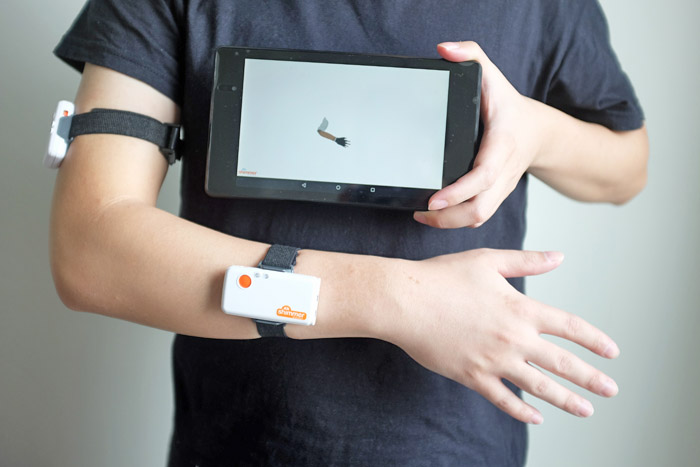
\includegraphics[scale=0.25]{Figures/Shimmer.jpg}
%  \caption{Wearable devices from the Shimmer platform.}
%  \label{fig:Shimmer}
%  \vspace{-0.3cm}
%\end{figure}
%
%
%All results collected and analyzed in this paper were obtained based on the energy consumption of wireless wearable devices (nodes), model 2R, produced by the company Shimmer~\cite{burns2010shimmer}. These instruments provide the collection of vital signs of patients through sensors, such as accelerometer, magnetometer, gyroscope, among others. Once collected, vital signs should be transferred to other more efficiently computational devices known as wireless body network coordinators. This transmission can be performed in two ways. The first one takes place directly, using Bluetooth technology. While the other mode would be with the aid of retransmission devices using ZigBee radio, since they provide better energy efficiency. 
%
%Os softwares que desenvolvemos para emular o monitoramento de sinais vitais, aplicados aos nós sensores Shimmer foram projetados com auxílio da linguagem de programação NesC~\cite{gay2014nesc}, a qual é baseada na linguagem C. Esta também é a linguagem adotada para o desenvolvimento do RTOS ({\em Real Time Operating System}), utilizado pelos nós sensores, e pelo Tinyos~\cite{levis2005tinyos}, o qual é um sistema operacional completamente voltado para aplicações em sistemas embarcados, permitindo a criação e a extensão de componentes específicos para cada característica de nó sensor.
%
%The NesC programming language is the basis for software development to these devices and for the RTOS (Real Time Operating System) running 
%Devices rely on a software developed in NesC programming language to %emulate the
%monitor vital signs. % applied to Shimmer sensor nodes was designed with the programming language NesC~\cite{gay2014nesc}, which is based on the C language. 
%NesC is also the basis for the %This is also the programming  language adopted for the 
%development of the RTOS (Real Time Operating System) running %on the wearable devices 
%together to TinyOS, %~\cite{levis2005tinyos},
%which is an operating system completely geared towards applications in embedded systems, allowing the creation and extension of components specific for each wearable device feature.


Energy consumption is measured in three different states (i.e., idle, sleep and run). At a glance, we set up the wearable to the desired state and continuously monitor it. The wearable device is automatically placed in a low-power mode when the task queue is empty (\textit{idle}: state 1). We can manually adjust the microprocessor for sleep mode (\textit{sleep}: state 2). In this sense, we are able to measure the wearable device lower level of power consumption. Finally, to monitor the wearable device on run state, we setup device to continuously perform a cryptography task ---on 64-bits data blocks--- using one of the aforementioned cryptography algorithms, followed by the encrypted data transmission using ZigBee (run: state 3) or Bluetooth (run: state 4).
Finally, unless we tell otherwise, at each state we perform 2000 samples and present mean confidence interval (for 95\% confidence level).


\begin{figure}[tbh]
 %\vspace{-0.3cm}
  \centering
  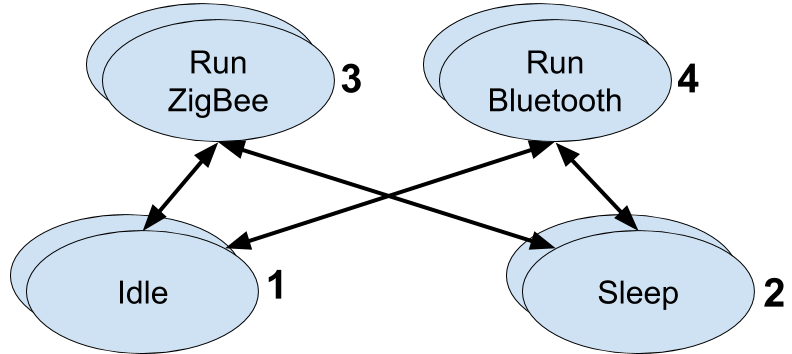
\includegraphics[scale=0.19]{Figures/estados.png}
  \caption{Wearable device states}
  \label{fig:states}
  \vspace{-0.1cm}
\end{figure}

We have designed and assembled a circuit for energy consumption measurement adapted from~\cite{bessa2017jetsonleap}. The circuit comprises of a low cost data acquisition board\footnote{DAQ - ADALM1000} connected to a wearable device, a 0.10~\si{\ohm} resistor, and a computer (Figure~\ref{fig:circuit}).
We use Active Learning Interface for Circuits and Electronics (ALICE) software to acquire voltage measurements from both terminals of the resistor which are connected to channels CH\_A and CH\_B of the DAQ. The voltage can be easily transformed to current following the law of Ohm, $V = R$ x $I$, since the resistance value is known. In order to make comparisons possible, we finally calculate the power consumption by multiplying the current to the voltage. Then, power consumption follows: 
$P = ((\mbox{CH\_A} - \mbox{CH\_B}) / 0.10) * V $ mW.



\begin{figure}[!htb]
 \vspace{-0.1cm}
  \centering
  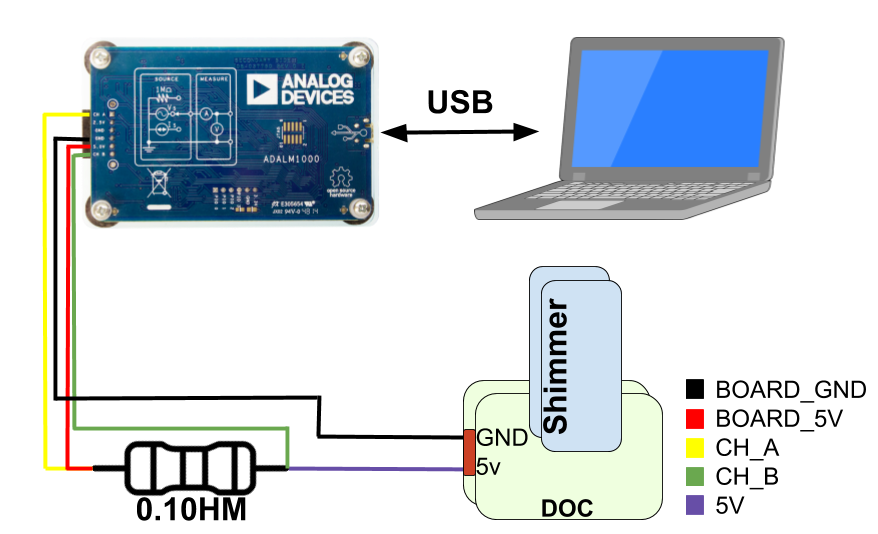
\includegraphics[scale=0.19]{Figures/circuit.png}
  \caption{Energy consumption measurement}
  \label{fig:circuit}
  %\vspace{-0.3cm}
\end{figure}

DAQ delivers a maximum sampling rate of 100 ksps (kilosamples per second).
 Therefore, we 
calculate energy consumption, mean, and the total consumption time for the algorithms in each analyzed state of wearable devices. Also, the computational complexity of the algorithms is of great relevance because energy consumption bottlenecks occur during data processing and transmission. Hence,  We also consider 
the size of machine code, since this represents a large share of the hardware resource consumption.


In addition to energy consumption, we analyze the main operations in each cryptography algorithm.
Hence, we
enumerate all the logical and arithmetic operations, once we want to confirm if the number of operations can be directly correlated with the final performance and energy consumption for the implementation of each algorithm.
Further, since wearable devices are severely constrained in computational resources, we also analyze the amount of memory the implementation of each algorithm consumes. We extract this information with the help of the NesC compiler.


\label{sec:Methodology}

%The experiments in this letter rely on wearable devices from the Shimmer platform, model 2R. These devices sense vital signs and movements from users by accelerometers, magnetometers, and gyroscope, and transmit them to a coordinator device (e.g., a smartphone) through wireless communication, such as Bluetooth or Zigbee. These devices run the Real Time Operating System (RTOS) together to TinyOS. NesC is the programming language for software development, including the operating system. 

%The experiments in this letter rely on wearable devices from the Shimmer platform for clinical trials, model 2R. These devices are equipped with a MSP430 F1611 microcontroller, 16-bit RISC architecture. \rever{Each device contains 48KB flash memory and 10KB RAM.} These devices sense vital signs and movements from users by accelerometers, magnetometers, and gyroscope, and transmit them to a coordinator device ({\em e.g.}, a smartphone) through wireless communication, such as Bluetooth or Zigbee. The Shimmer platform employs the Roving Networks RN-42, a low-cost and low-power Bluetooth module. The Zigbee module follows the CC2420 radio transceiver, designed for size-constrained, low-power and low-current applications. \rever{These low-power wireless devices run the Real-Time Operating System (RTOS), known as TinyOS.}

\rever{In this work, the experiments rely on two platforms: % The first,
$(i)$ wearable devices from the Shimmer platform, model 2R %~\cite{shimmer}
and $(ii)$ a Teensy\texttrademark~3.2 microcontroller. The Shimmer devices are equipped with a MSP430 F1611 microcontroller, 16-bit RISC architecture. Each wearable device contains 48KB flash memory and 10KB RAM. These devices sense vital signs and movements from users by accelerometers, magnetometers, and gyroscope, and transmit them to a coordinator device ({\em e.g.}, a smartphone) through wireless communication. These low-power wireless devices run TinyOS, a Real-Time Operating System (RTOS). The Teensy platform is equipped with an ARM\textsuperscript{\textregistered} Cortex\textsuperscript{\textregistered}-M4 of 72 MHz CPU and 32-bit architecture. This device also contains a 256KB flash memory and 64KB RAM memory. For Teensy, the algorithms were implemented in C language and deployed using the Arduino interface.} %\rever{\cite{shimmer}}

%Power consumption is measured in different states ({\em i.e.}, idle, and run). At a glance, we set up the devices to the desired state and continuously monitor it. The devices is automatically placed in a low-power mode when the task queue is empty (\textit{idle}: state 1). We can manually adjust the microprocessor for sleep mode (\textit{sleep}: state 2). In this sense, we are able to measure the wearable device power consumption. Finally, to analyze the wearable on run state, we setup the device to continuously perform a cryptography task --- on 64-bits data blocks --- using one of the aforementioned cryptography algorithms, followed by the encrypted data transmission using ZigBee ({\em run:} state 3) or Bluetooth ({\em run:} state 4). Finally, unless we tell otherwise, at each state we perform 2,000 samples and present mean confidence interval of 95\%.

\rever{We measure power consumption in different states ({\em i.e.}, idle, and run). At a glance, we set up the devices to the desired state and continuously monitor it. The devices are automatically placed in a low-power mode when the task queue is empty (\textit{idle} state). Hence, we are able to measure the device power consumption in this state. Finally, to analyze the wearable on the run state, we set up the device to continuously perform a cryptography task --- on 64-bits data blocks --- using one of the aforementioned cryptography algorithms on both platforms, {\em run} state). In the Shimmer platform, {\em run} state, we consider the cost of encrypted data transmission. Finally, unless we tell otherwise, at each state we perform 2,000 samples and present mean confidence interval of 95\%.}

% \begin{figure}[tbh]
% \vspace{-0.3cm}
%  \centering
%  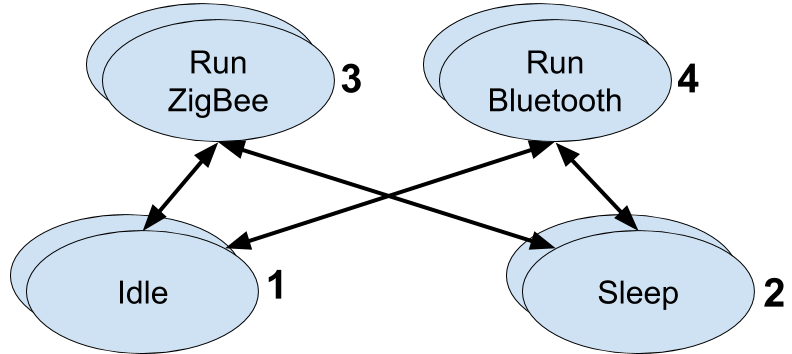
\includegraphics[scale=0.19]{Figures/estados.png}
%  \caption{Wearable device states}
%  \label{fig:states}
%  \vspace{-0.5cm}
% \end{figure}

We have designed and assembled a circuit for power consumption measurement adapted from~\cite{bessa2017jetsonleap}. The circuit comprises of a low-cost data acquisition board (DAQ - ADALM1000) connected to a wearable, a 0.10~\si{\ohm} resistor, and a computer (Figure~\ref{fig:circuit}). We use Active Learning Interface for Circuits and Electronics (ALICE) software to acquire voltage measurements from both terminals of the resistor which are connected to channels CH\_A and CH\_B of the DAQ. The voltage can be easily transformed to current following the law of Ohm, $V = R$ x $I$, since the resistance value is known. 
To make comparisons, we calculate the power consumption by multiplying the current to the voltage. Then, power consumption follows: 
$P = ((\mbox{CH\_A} - \mbox{CH\_B}) / 0.10) * V $ mW.

\begin{figure}[!htb]
 \vspace{-0.3cm}
 \centering
 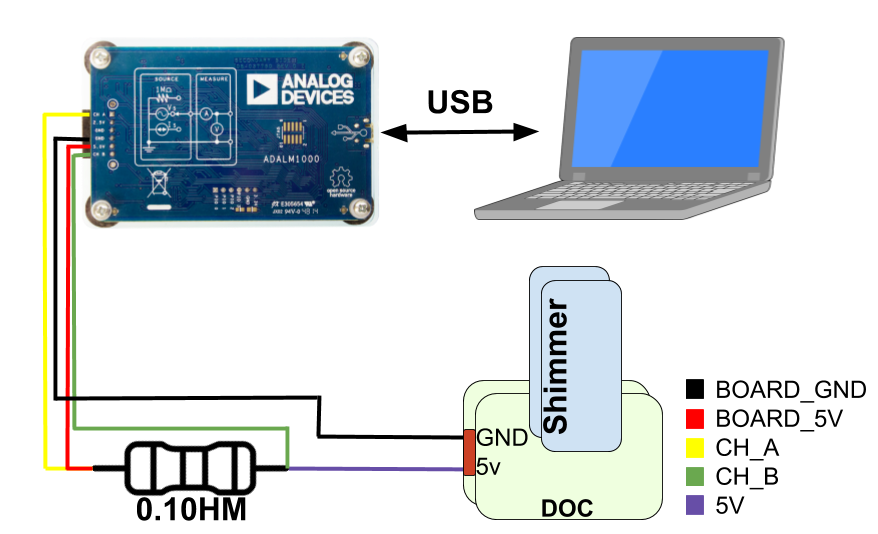
\includegraphics[scale=0.19]{Figures/circuit.png}
 \caption{Power consumption measurement}
 \label{fig:circuit}
 \vspace{-0.3cm}
\end{figure}

DAQ delivers a maximum sampling rate of 100 ksps (kilosamples per second). Therefore, we calculate power consumption, mean, and the total consumption time for the algorithms in each analyzed state of wearable devices. Also, the computational complexity of the algorithms is of great relevance because power consumption bottlenecks occur during data processing and transmission. Hence, we also consider the size of machine code, when it represents a large share of the hardware resource consumption.

%\rever{In addition to energy consumption, We have counted the number of Assembly instructions with the help of the Godbolt online compiler and a manual process known as Table Test. The Godbolt compiler converts programs from several languages into Assembly code. For the experiment we use the MSP430 GCC compiler \cite{MSPGCC} version 5.3.0 without optimization directives and then we convert the NesC code to Assembly code. Next, using the Table Test we have counted the final number of Assembly instructions.}

\rever{%In addition to power consumption, 
We also count the number of Assembly instructions using the Godbolt online compiler and a manual process known as Table Test. The Godbolt compiler converts programs from several languages into Assembly code. For the experiment, we use the MSP430 GCC compiler version 5.3.0 %~\cite{MSPGCC} 
for Shimmer platform and AVR GCC version 4.6.4 for Teensy platform, both without optimization directives. Then, we convert the %cryptography algorithm 
code to Assembly code. Next, using the Table Test, we have counted the final number of Assembly instructions.}

\rever{Similarly, we also analyze the main operations in each cryptography algorithm. The considered operations are {\em shift left, shift right, and, or, not, xor, sum, subtraction}, and {\em multiplication}. We enumerate all these logical and arithmetic operations when we want to confirm if the number of operations can be directly correlated with the final performance and power consumption of each algorithm implementation~\cite{mohd2018lightweight}. Furthermore, since wearable devices are severely constrained in computational resources \rever{, and implantable devices have hard limitations for replacement}, we analyze the amount of memory the implementation of each algorithm requires. We derive this information to memory consumption (ROM and RAM separately) of each cryptography algorithm using MSPGCC compiler for Shimmer platform and AVR GCC for Teensy platform~\cite{cazorla2013survey}. %~\cite{MSPGCC,cazorla2013survey}. 
To ensure equivalence between measurements, we disregard the overhead produced by TinyOS on the Shimmer platform. Hence, we can assert that the presented data refers exactly to each algorithm.}

%\rever{Analogously, we still analyze the main operations in each cryptographic algorithm. We enumerate all the logical and arithmetic operations, when we want to confirm if the number of operations can be directly correlated with the final performance and energy consumption of each algorithm implementation~\cite{mohd2018lightweight}. Furthermore, since wearable devices are severely constrained in computational resources, we analyze the amount of memory the implementation of each algorithm requires. We derive this information to memory consumption (ROM and RAM separately) of each cryptography algorithms using MSPGCC compiler with debug flags enabled~\cite{MSPGCC,cazorla2013survey}. To collect such information, we have compiled the implementation of each cryptographic algorithm independently of any other function directed to the platform Shimmer2r. Hence, we can assert that the presented data refers exactly to each algorithm.}


\vspace{-0.3cm}
\section{Results}
\label{sec:Results}
%
Power dissipation is one of the critical factors for the development of wearable networks for high-end and low-end embedded devices. Therefore, a wide energy efficiency analysis, evaluating different factors in the design of the wearable devices, has great relevance. 
In a PSM, states are the modes of operation of the device. A transition between two states represents the energy cost and the delay spent consolidating state change. Thus, low power  states  have  a  longer  delay  between  transitions for states Run. The transition  time  is presented in~\cite{goraczko2008energy}, where it still infers that the times of the other transitions are insignificant and for the matter of simplicity not represented in the PSM.


Figure~\ref{fig:PSM_geral} represents the PSM of the wearable device we analyze in this work. %As we discussed in Section~\ref{sec:Methodology}, the wearable device presents three main states (idle, sleep and run). For the matter of simplicity, we have omitted in this figure transitions with negligible delays (e.g., Idle $\leftrightarrow$ Sleep). %According to this figure, 
Regardless the transmission mode on run state (i.e., ZigBee or Bluetooth), the sleep and idle states of the device present a mean energy consumption of 226.95\,mW and 236.21\,mW, respectively. The difference is of only 4.08\%, because wearable devices are automatically placed in low-power mode when they are not performing tasks. The sleep state presents a slightly higher transition time than the run state, when compared to the transition between the idle and run states. Thus, the fact that the idle state automatically operates at low power makes it attractive for exempting the developer from managing different sleep levels and their interruptions. 


\begin{figure}[tbh]
% \vspace{-0.3cm}
  \centering
  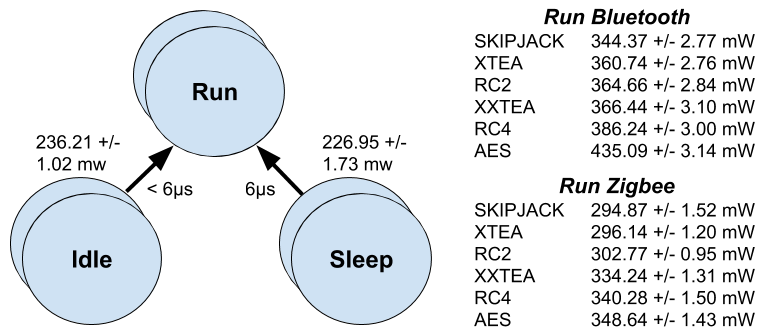
\includegraphics[scale=0.3]{Figures/C_PSM_geral.png}
  \caption{Wearable device power state machine (PSM)}
  \label{fig:PSM_geral}
 % \vspace{-0.3cm}
\end{figure}

\begin{figure*}[!t]
  %\vspace{-0.5cm}
\centering
  \begin{subfigure}[b]{0.4\textwidth}
    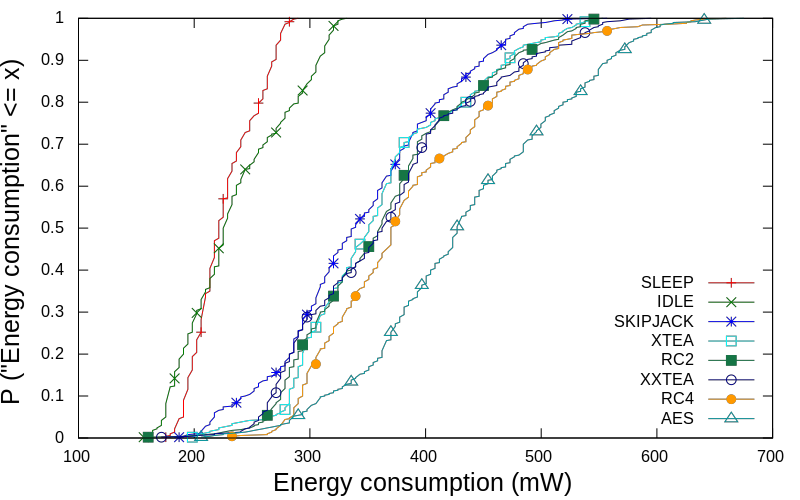
\includegraphics[width=\textwidth]{Figures/cdf_blue_aes.png}
    \caption{Power consumption per state using Bluetooth}
    \label{fig:cdf_blue}
  \end{subfigure}
  %
  \begin{subfigure}[b]{0.4\textwidth}
    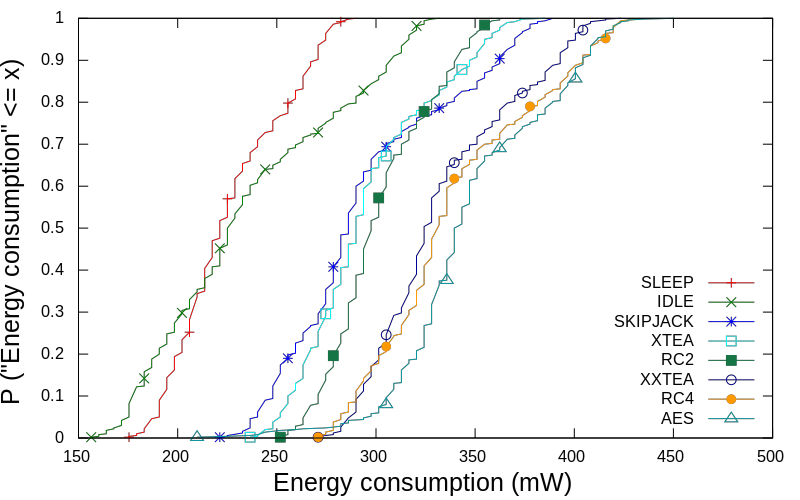
\includegraphics[width=\textwidth]{Figures/cdf_zig_aes.png}
    \caption{Power consumption per state using ZigBee}
    \label{fig:cdf_zig}
  \end{subfigure}
  \caption{Energy consumption on the run state}
  \vspace{-0.3cm}
\end{figure*}

Moreover, the run state, which encompasses data processing and transmission, asymptotically dominate energy consumption.  
For example, the run state using Bluetooth spends up to 71\% more energy, in the worst case, than the idle state. Clearly, for both transmission standards, SKIPJACK presents the lowest energy consumption among the evaluated algorithms. SKIPJACK, associated with Bluetooth or Zigbee, spends 12.16\% to 15.4\% less energy, respectively, than RC4 (which demands the highest amount of energy). Finally, ZigBee reduces the average energy consumption by 16.44\% when compared to Bluetooth.


%%%%%%%%%%%%%%%%%%%%%%%%%%%%%%%%%%%%%%%%%%%%%%%%%%%
\begin{comment}
\begin{table}[ht]
\centering
\caption{PSM Summary.}
%\vspace{0.3cm}
\label{table:papers}
\begin{tabular}{lccc}
\hline
\multicolumn{3}{c}{Transition latency}\\
\hline
Idle-Run & \multicolumn{2}{c}{$<$6us}\\
Sleep-Ru  & \multicolumn{2}{c}{6us}\\
\hline
\multicolumn{3}{c}{Energy Consumption}\\
\hline
Idle & \multicolumn{2}{c}{47.242}\\
Sleep & \multicolumn{2}{c}{45.390}\\
Run &  Bluetooth & Zigbee  \\
 \hline
SKIPJACK & 68.873 & 58.875 \\
XTEA  & 72.148 & 59.226 \\
RC2 & 72.931 & 60.554\\
XXTEA & 73.288 &  66.847\\
RC4 & 77.247 & 68.055
\end{tabular}
\end{table}

\end{comment}
%%%%%%%%%%%%%%%%%%%%%%%%%%%%%%%%%%%%%%%%%%%%%%%%%%

\begin{comment}
\begin{figure}[H]
 \vspace{-0.5cm}
  \centering
  \includegraphics[scale=0.25]{Figures/PSM_ZB.png}
  \caption{Power State Machine (PSM) using ZigBee.}
  \label{fig:PSM_ZB}
  %\vspace{-0.5cm}
\end{figure}
\end{comment}


%As Figuras~\ref{fig:cdf_blue} e~\ref{fig:cdf_zig} descrevem completamente a distribuição da probabilidade representado todos os cenários avaliados. A primeira referência a aplicação usando Bluetooth enquanto a segunda utiliza ZigBee. Deste modo, é possível notar que o comportamento do consumo dos métodos criptográficos ratificam os resultados apresentados pelo consumo médio. Com isto inferimos o Skipjack como método mais eficiente, opondo-se ao RC4, quando seu uso apresenta maior dissipação de energia.

Figures~\ref{fig:cdf_blue} and~\ref{fig:cdf_zig} %\abv{further 
detail the  energy consumption per state and  present the Cumulative Distribution Function (CDF) for each evaluated scenario. Figure~\ref{fig:cdf_blue} shows results when using Bluetooth, whereas Figure~\ref{fig:cdf_zig} presents results for the use of ZigBee. %It is possible to notice that 
Results for energy consumption following each cryptograph algorithm ratify the average energy consumption %\abv{
per state in Figure~\ref{fig:PSM_geral}. % and \ref{fig:PSM_ZB}. %  results presented by the average energy consumption. 
%Therefore, 
We observe SKIPJACK as the most efficient among all evaluated algorithms, and RC4 the least. % opposing RC4, when its use presents greater energy dissipation.

\begin{comment}
\begin{figure}[H]
  \centering
  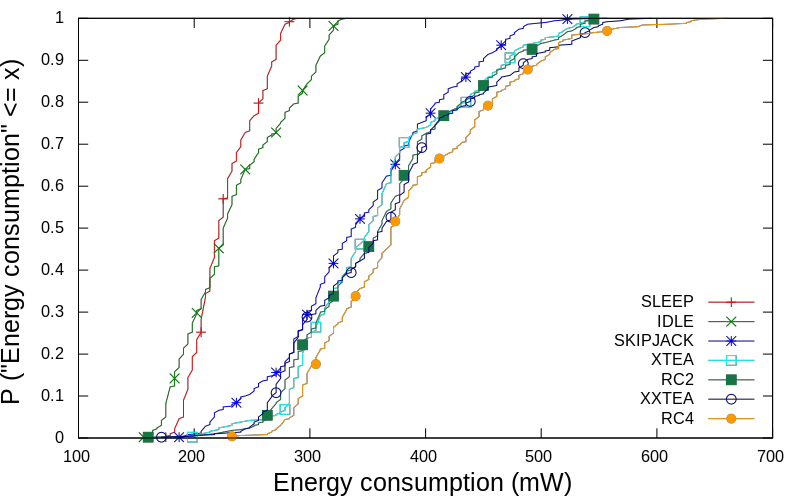
\includegraphics[scale=0.32]{Figures/cdf_blue_.png}
  \caption{Cumulative Distribution Function for energy consumption by state using Bluetooth.}
  \label{fig:cdf_blue}
\end{figure}

\begin{figure}[H]
  \centering
  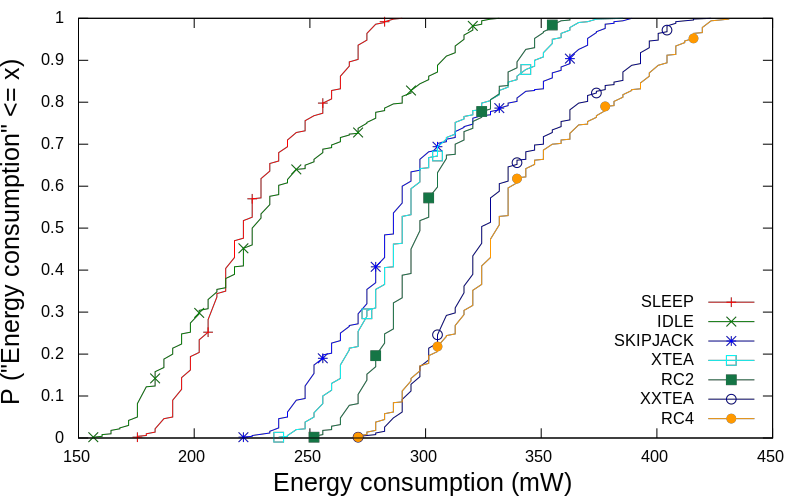
\includegraphics[scale=0.32]{Figures/cdf_zig_.png}
  \caption{Cumulative Distribution Function for energy consumption by state using ZigBee.}
  \label{fig:cdf_zig}
\end{figure}

\end{comment}



%%%%%%%%%%%%%%%%%%%%%%%%%%%%%%%%%%%%%%%%%%%%%%%%%%%%%%%%
%%%%%%%%%%%%% texto antigo    do inicio da seção %%%%%%%
%%%%%%%%%%%%%%%%%%%%%%%%%%%%%%%%%%%%%%%%%%%%%%%%%%%%%%%%
\begin{comment}
%A dissipação de energia é um dos fatores críticos para o desenvolvimento de sistemas para dispositivos embarcados de ponta e de baixo custo. Portanto uma análise de eficiência energética ampla, avaliando fatores distintos no projeto dos nós sensores possui grande relevância. Deste modo podemos representar os estados do nó com uma máquina de estado de potência (PSM), onde os estados são os modos de operação dos nós. As transições entre estados têm custo de energia e atraso. Assim, os modos de baixo consumo possuem maior atraso nas transições~\cite{benini2000survey}. Entretanto, algumas vezes este atraso pode ser insignificante.

Power dissipation is one of the critical factors for the development of wearable networks for high-end and low-end embedded devices. Therefore, a wide energy efficiency analysis, evaluating different factors in the design of the wearable devices, has great relevance. Hence, we represent the states of a given wearable device by a power state machine (PSM), where states are the modes of operation of the device. Transitions between states have energy cost and delay. Thus, low power modes have a longer delay in transitions~\cite{benini2000survey}, noting that sometimes this delay can be insignificant.

%Apoiando-se nisso, apresentamos um modelo abstrato simples do PSM para o nó sensor vestível e seus principais modos de atividade. O modo de processamento e a transmissão dos dados domina assintoticamente o consumo energético. Este, juntamente com os modos~\textit{idle} e~\textit{sleep}, representam os principais estados do nó na rede. Assim, a Figura~\ref{fig:PSM_BLUE} representa o PSM para o nó utilizando a transmissão de dados via Bluetooth. Por meio desta, podemos observar os estados com seus respectivos valores de dissipação de potência e as arestas de transição de estados e seus tempos. Este tempo referente às transições é apresentado em~\cite{goraczko2008energy}, onde ainda infere que os tempos das demais transições são insignificantes e por isso não representadas no PSM.


Figure~\ref{fig:PSM_geral} represents the PSM for \abv{a given wearable device} using Bluetooth for data transmission. We present a simple abstract model of PSM for a wearable device and its main states. Processing and data transmission modes asymptotically dominate energy consumption. This, along with the idle and sleep states, represents the major states of a wearable device in the network. In the figure, we observe the states with their respective values for power dissipation, state transitions and their times. Transition time follows~\cite{goraczko2008energy}, where it still infers that the times of the other transitions are insignificant and therefore not represented in the PSM, (e.g., Idle $\leftrightarrow$ Sleep).


\begin{figure}[tbh]
  \vspace{-0.3cm}
  \centering
  \includegraphics[scale=0.23]{Figures/PSM_blue.png}
  \caption{Power State Machine (PSM) using Bluetooth.}
  \label{fig:PSM_BLUE}
  \vspace{-0.2cm}
\end{figure}

%Observe que o modo~\textit{sleep} apresenta um menor consumo médio, 45.390 mA, contra 47.242 mA do modo~\textit{idle}. O que representa uma diferença de apenas 4,08\%. A estreita disparidade é justificada pelo fato do nó, automaticamente ser colocado em modo de baixa potência quando não está a executar tarefas. O modo~\textit{sleep} ainda apresenta tempo de transição levemente superior. Deste modo, o fato do modo~\textit{idle} operar em baixa potência automaticamente torna seu uso atraente. Isto pelo fato de isentar o desenvolvedor da função de gerenciar os diversos níveis de sono, bem como suas interrupções. Entre os algoritmos de criptografia a diferença no consumo médio chegou a 12.16\%. Destaque para o método SKIPJACK que se mostrou mais eficiente, em contraposição ao RC4.

%Note that 
Sleep mode has the lowest average energy consumption, 45,390 mA, compared to 47,242 mA in the idle mode. The difference is of % represents a difference  
only 4.08\%, because wearable devices are 
%
%The narrow difference is justified by the fact that the node is 
automatically placed in low power mode when they are not performing tasks. The sleep mode still has slightly higher transition time \abv{to running mode? falta um complemento na frase}. Thus, the fact that idle state automatically operates at low power makes it attractive for exempting the developer from managing different sleep levels and their interruptions. 
%
%. This is because it exempts the developer from the function of managing the various sleep levels, as well as their interruptions. 
Among the evaluated algorithms the difference of energy consumption, in average, reaches 12.16\%, highlighting SKIPJACK as the algorithm with the lowest energy consumption. %  more efficient, as opposed to RC4.

%De modo análogo, a Figura~\ref{fig:PSM_ZB}, proporciona a análise do consumo médio utilizando ZigBee como tecnologia de transmissão de dados. Deste modo, novamente destaca-se o método SKIPJACK como mais eficiente, dispondo de uma diferença de aproximadamente 15.4\% perante o método RC4. A partir destes dados podemos inferir também que optar por utilizar ZigBee como tecnologia de transmissão de dados proporciona uma eficiência energética média, na casa de 16.44\% em relação ao Bluetooth na média.

%Similarly, 
Figure~\ref{fig:PSM_ZB} provides the average energy consumption analysis when the wearable device uses ZigBee for data transmission. Again, SKIPJACK presents the lowest energy consumption, with a difference of approximately 15.4\% compared to RC4. We infer that ZigBee reduces the average energy consumption in 16.44\% compared to Bluetooth.

\end{comment}

\rever{Power consumption is one of the critical factors in the design and development of wearable networks for both high-end and low-end embedded devices. Therefore, a comprehensive power efficiency analysis, considering all possible factors is of great relevance.} A Power State Machine (PSM) represents the possible states of a device, and a transition between two states means power cost and delay.
Thus, low power states have a longer delay between transitions for {\em run} states. The transition time is presented in~\cite{goraczko2008energy}. The time for other transitions is considered insignificant and %, for the sake of simplicity,
it is not represented in PSM.


%Figure~\ref{fig:PSM_geral} represents the PSM of the wearable device we analyze in this work. Regardless the transmission mode on {\em run} state ({\em i.e.} ZigBee or Bluetooth), the {\em sleep} and {\em idle} states of the device present a mean energy consumption of 226.95\,mW and 236.21\,mW, respectively. The difference is of only 4.08\%, because wearable devices are automatically placed in low-power mode when they are not performing tasks. The {\em sleep} state presents a slightly higher transition time than the {\em run} state, when compared to the transition between the {\em idle} and {\em run} states. Thus, the fact that the {\em idle} state automatically operates at low power makes it attractive for relieving the developer from managing different sleep levels and their interruptions. 

%\rever{Figure~\ref{fig:PSM_geral} represents the PSM of the devices we analyze in this work. In the {\em idle} state, this platforms automatically operates at low power makes it attractive for relieving the developer from managing different sleep levels and their interruptions.}

\rever{Figure~\ref{fig:PSM_geral} represents the PSM of the evaluated devices. In the {\em idle} state, the employed platforms run automatically under low energy consumption, being attractive because they manage themselves the different levels of suspension and interruptions, which makes easier for the developer. The figure also presents the average power consumption for each cryptographic algorithm and evaluated state and the transition time between states. Thus, we highlight the SKIPJACK algorithm, that improves energy efficiency in 18\% compared to AES.}

%\refazer{A figura~\ref{fig:PSM_geral} representa o PSM dos dispositivos que analisamos neste trabalho. No estado {\em idle}, essas platformas operam automaticamente com baixo consumo de energia, o que o torna atraente para aliviar o desenvolvedor de gerenciar diferentes níveis de suspensão e suas interrupções. A figura apresenta ainda informações relativas ao consumo médio de energia no estado {\em run} de cada algoritmo criptográfico para cada estado avaliado, bem como tempo de transição entre estados. Deste modo, é considerável listar a eficiência energética do algoritmo SKIPJACK, superior a 18\% em ambas platformas, quando confrontado com o AES.}

\begin{figure}[tbh]
 \vspace{-0.3cm}
 \centering
 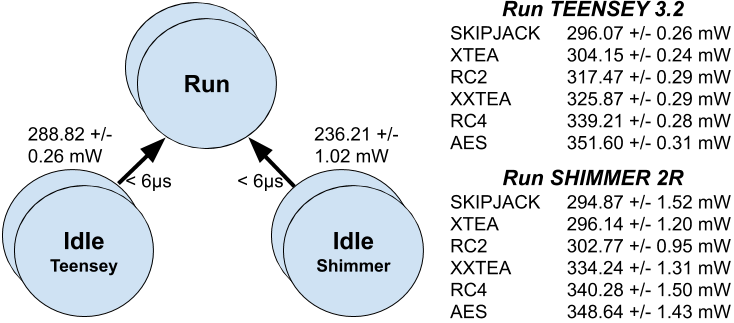
\includegraphics[scale=0.3]{Figures/PSM_Geral.png}
 \caption{\rever{Wearable device power state machine (PSM)}}
 \label{fig:PSM_geral}
 \vspace{-0.3cm}
\end{figure}

\begin{figure*}[!t]
 \vspace{-0.5cm}
\centering
 \begin{subfigure}[b]{0.35\textwidth}
  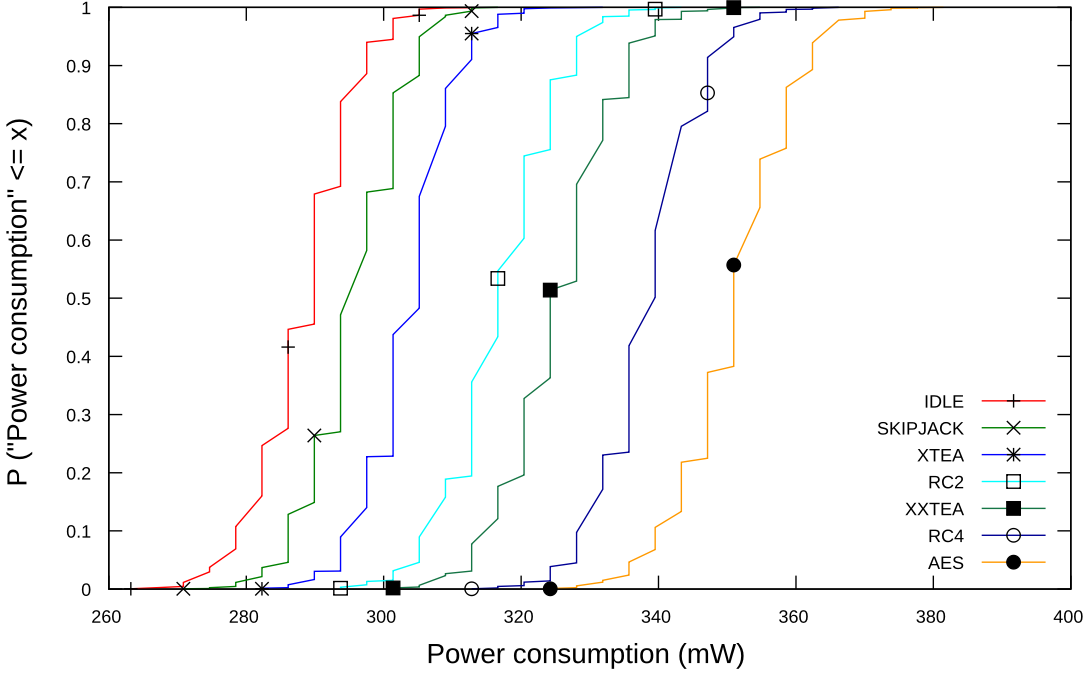
\includegraphics[width=\textwidth]{Figures/cdf_Teensy.png}
  \caption{\rever{Power consumption per state Teensy 3.2}}
  \label{fig:cdf_Teensy}
 \end{subfigure}
 \hspace{10mm}
 \begin{subfigure}[b]{0.35\textwidth}
  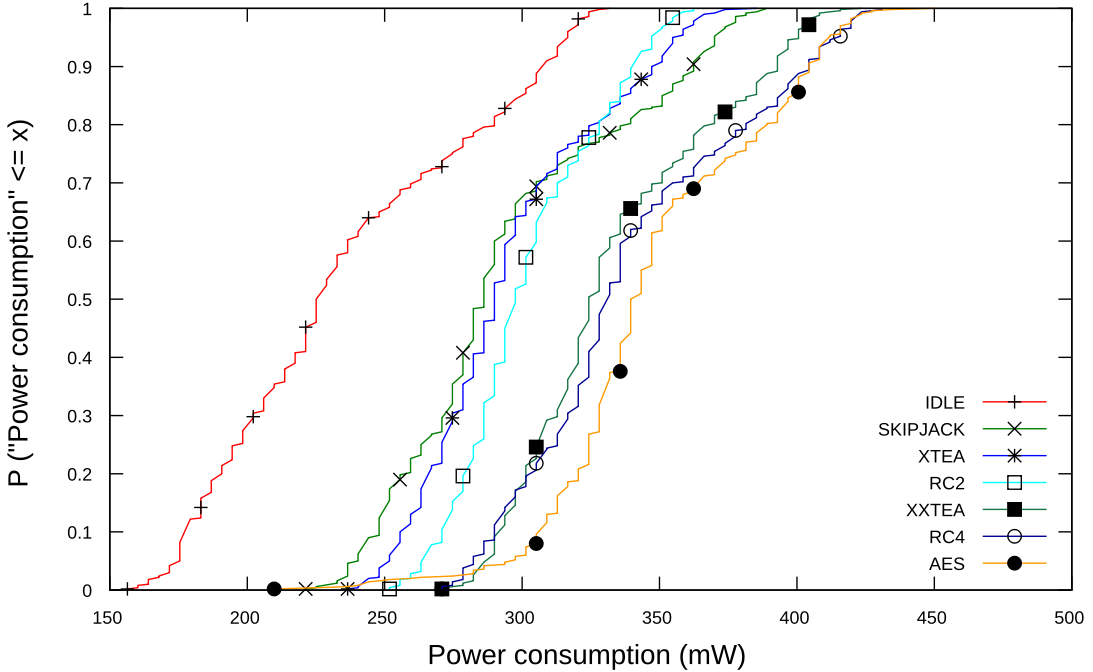
\includegraphics[width=\textwidth]{Figures/cdf_zig.png}
  \caption{\rever{Power consumption per state Shimmer 2R}}
  \label{fig:cdf_zig}
 \end{subfigure}
 \vspace{-0.2cm}
 \caption{\rever{Power consumption in milliwatts on the {\em run} state}}
 \label{fig:cdf}
 \vspace{-0.45cm}
\end{figure*}

\rever{The {\em run} state asymptotically dominates energy consumption. The analysis of power consumption for the Shimmer platform includes cryptographic processing and radio data transmission. With the Teensey platform, we have excluded the transmission operation and we can observe a similarity in the allusive behavior to the energy consumption of the cryptographic algorithms. Figure~\ref{fig:cdf} shows the behavior of the evaluated algorithms in both platforms through the Cumulative Distribution Functions (CDFs). Figure~\ref{fig:cdf_Teensy} illustrates the results for the Teensy platform, and Figure~\ref{fig:cdf_zig} presents results for the Shimmer platform.}

%\refazer{O estado {\em run}, domina assintoticamente o consumo de energia. Durante a análise para platforma Shimmer os dados referente ao consumo de energia incluem processamento criptográfico e a transmissão dos dados via rádio. Com o Teensey, excluímos a tecnologia de transmissão e podemos observar uma similaridade no comportamento alusivo ao consumo energético dos algoritmos criptográficos. A Figura~\ref{fig:cdf} exibe o comportamento dos algoritmos avaliados em ambas platformas apresentados em Função de Distribuição Cumulativa (CDF). A Figura~\ref{fig:cdf_Teensy} ilustra os resultados da platforma Teensy, enquanto a Figura~\ref{fig:cdf_zig} apresenta resultados para o uso da platforma comercial Shimmer.}

%18.76\% Teensy
%18.24\% Shimmer

%\refazer{The {\em run} state, which encompasses data processing and transmission, asymptotically dominate power consumption. For example, the {\em run} state using Bluetooth spends up to 84\% more energy than the {\em idle} state, , in the worst case. Clearly, for both communication standards, SKIPJACK presents the lowest energy consumption among the evaluated algorithms. SKIPJACK, associated with Bluetooth or Zigbee, spends 30.12\% to 17.56\% less energy, respectively, than AES (which demands the highest amount of energy). Finally, ZigBee reduces the average energy consumption by 17.37\% compared to Bluetooth.}

%\rever{Figures~\ref{fig:cdf_Teensy} and~\ref{fig:cdf_zig} detail the power consumption per state and present the Cumulative Distribution Function (CDF) for each evaluated scenario in both platforms. Figure~\ref{fig:cdf_Teensy} shows results for Teensy platform, whereas Figure~\ref{fig:cdf_zig} presents results for the use of commercial platform Shimmer. Results for power consumption following each cryptographic algorithm showing the average power consumption per state are summarized in Figure~\ref{fig:PSM_geral}. SKIPJACK is the most efficient among all evaluated algorithms, and AES the least.} 



%We again have a positive observation for SKIPJACK, that presented fewer operations to encrypt a 64-bit data block. \rever{The Table~\ref{tab:comp} also shows information about memory use (including ROM and RAM usage). We note a low difference in total resource allocation (about 3.85\%) between XTEA and SKIPJACK.}

% Please add the following required packages to your document preamble:
% \usepackage{multirow}

\rever{The computational cost of logical and arithmetic operations has a direct effect on processing time and wearable device power consumption. Table~\ref{tab:comp} shows the number of operations for each evaluated algorithm and their respective complexity. The count is relative to the encryption function, once the wearable device performs this function, but not decryption. Thus, power consumption has a direct correlation with the number of operations. Another correspondence observed is the proportionality of ROM/RAM occupancy between the algorithms, $\approx11$\%. In addition to finding a ROM memory consumption about $\approx3.5$x higher of AES in relation to SKIPJACK, considering the Shimmer platform.}

\begin{table}[h!]
\scriptsize
\centering
 \setlength\tabcolsep{7.7 pt} % default value: 6pt
\vspace{-0.1cm}
\caption{\rever{Computational complexity vs. memory consumption}}
\vspace{-0.2cm}
\begin{tabular}{l|c|ccll}
\hline

\multirow{3}{*}{ALGORITHM} & \multirow{3}{*}{\begin{tabular}[c]{@{}c@{}}COMPLEXITY\end{tabular}} &\multicolumn{4}{c}{\begin{tabular}[c]{@{}c@{}}\rever{MEMORY CONSUMPTION (BYTES)}\end{tabular}}\\ \cline{3-6} 
          &                 & \multicolumn{2}{c|}{\rever{Shimmer 2R}}                               & \multicolumn{2}{c}{\rever{Teensy 3.2}}    \\ \cline{3-6} 
            &               & \multicolumn{1}{c|}{\rever{ROM}}  & \multicolumn{1}{c|}{\rever{RAM}}  & \multicolumn{1}{c|}{\rever{ROM}}  & \rever{RAM}  \\ \hline
SKIPJACK    & $O(1)$        & \multicolumn{1}{c|}{\rever{6,834}}        & \multicolumn{1}{c|}{\rever{608}}          & \multicolumn{1}{l|}{\rever{13,892}}       & \rever{4,584} \\
XTEA        & $O(1)$        & \multicolumn{1}{c|}{\rever{6,772}}        & \multicolumn{1}{c|}{\rever{612}}          & \multicolumn{1}{l|}{\rever{13,360}}       & \rever{4,620} \\
RC2         & $O(1)$        & \multicolumn{1}{c|}{\rever{6,786}}        & \multicolumn{1}{c|}{\rever{726}}          & \multicolumn{1}{l|}{\rever{14,028}}       & \rever{4,828} \\
XXTEA       & $O(n)$        & \multicolumn{1}{c|}{\rever{7,064}}        & \multicolumn{1}{c|}{\rever{604}}          & \multicolumn{1}{l|}{\rever{13,456}}       & \rever{4,556} \\
RC4         & $O(n)$        & \multicolumn{1}{c|}{\rever{6,994}}        & \multicolumn{1}{c|}{\rever{604}}          & \multicolumn{1}{l|}{\rever{13,348}}       & \rever{4,556} \\
AES         & $O(1)$        & \multicolumn{1}{c|}{\rever{24,068}}       & \multicolumn{1}{c|}{\rever{1,978}}        & \multicolumn{1}{l|}{\rever{14,048}}       & \rever{4,812} \\ \hline
\end{tabular}
\label{tab:comp}
\vspace{-0.5cm}
\end{table}

% \begin{table}[]
% \scriptsize
% \centering
% % \setlength\tabcolsep{6 pt} % default value: 6pt
% %\vspace{-0.2cm}
% \caption{Computational cost of logical/arithmetic operations}
% \vspace{-0.2cm}
% \begin{tabular}{l|c|c|c|c}
% \hline
% \multirow{2}{*}{ALGORITHM} & \multirow{2}{*}{\begin{tabular}[c]{@{}c@{}}KEY SIZE\\ (BITS)\end{tabular}} & \multirow{2}{*}{\begin{tabular}[c]{@{}c@{}}NUMBER OF\\ OPERATIONS\end{tabular}} & \multicolumn{2}{c}{\begin{tabular}[c]{@{}c@{}}MEMORY\\ CONSUMPTION (BYTES)\end{tabular}} \\ \cline{4-5} 
%              &                                       &                                         & \multicolumn{1}{N|}{ROM}         & \multicolumn{1}{c}{RAM}          \\ \hline
% SKIPJACK          & 80                                      & 496                                       & 6,834                    & 608                     \\
% XTEA            & 128                                     & 576                                       & 6,772                    & 612                     \\
% RC2            & 128                                     & 804                                       & 6,786                    & 726                     \\
% XXTEA           & 128                                     & 1,490                                      & 7,064                    & 604                     \\
% RC4            & 128                                     & 1,992                                      & 6,994                    & 604                     \\
% AES            & 128                                     & 2,704                                      & 24,068                    & 1,978                    \\ \hline
% \end{tabular}
% \label{tab:comp}
% \vspace{-0.6cm}
% \end{table}



% \begin{table}[h!]
% \scriptsize
% \centering
% \setlength\tabcolsep{4 pt} % default value: 6pt
% \vspace{-0.2cm}
% \caption{Computational cost of logical/arithmetic operations}
% \vspace{-0.2cm}
% \begin{tabular}{l|c|c|c|c} 
% \hline
% ALGORITHM & \begin{tabular}[c]{@{}c@{}}KEY\\SIZE\\(BITS) \end{tabular} & \begin{tabular}[c]{@{}c@{}}NUMBER OF\\OPERATIONS \end{tabular} & \begin{tabular}[c]{@{}c@{}}ROM MEMORY\\CONSUMPTION\\ (BYTES) \end{tabular} & \begin{tabular}[c]{@{}c@{}}RAM MEMORY\\CONSUMPTION\\ (BYTES) \end{tabular} \\ 
% \hline
% SKIPJACK & 80 & 496 & 6834 & 608\\
% XTEA   & 128 & 576 & 6772 & 612\\
% RC2   & 128 & 804 & 6786 & 726\\
% XXTEA  & 128 & 1490 & 7064 & 604\\
% RC4   & 128 & 1992 & 6994 & 604\\
% AES   & 128 & 2704 & 24068 & 1978\\
% \hline
% \end{tabular}
% \label{tab:comp}
% \vspace{-0.3cm}
% \end{table}
%\refazer{***********************************************}

\rever{Table~\ref{tab:instr} displays information about the amount of logical/arithmetic operations and assembly instructions performed by each cryptographic algorithm. This allows us to draw a direct correlation between these parameters and energy consumption. Hence, we observe that the SKIPJACK algorithm performs fewer operations and, thus, fewer instructions ($\approx 32$x), requiring less hardware performance and less energy, particularly, when compared to AES.
}

%\refazer{A tabela~\ref{tab:instr} apresenta informações acerca da quantidade de operações lógicas/aritméticas e instruções assembly executadas por cada algoritmo criptográfico. O que nos permite traçar uma correlação direta entre estes parâmetros e o consumo de energia. Deste modo podemos observar que o algoritmo SKIPJACK executa menos operações e consequentemente menos instruções ($\approx32$x), assim exigindo menos desempenho do hardware e demandando menos energia, principalmente quando confrontado com o AES.}

%\refazer{The Table~\ref{tab:instr} ilustre a comparison between the number of the assembly instruction per round, as well as the number of rounds of each algorithm. Thus, enumerating how much assembly instructions are executed most of the time (MAIN LOOP). Table II also shows the total number the instructions, besides the asymptotic complexity of each algorithm.}


% Please add the following required packages to your document preamble:
% \usepackage{multirow}
\begin{table}[h!]
\centering
\scriptsize
\setlength\tabcolsep{3pt} % default value: 6pt
\vspace{-0.1cm}
\caption{\rever{Logic/arithmetic operations vs. assembly instructions}}
\vspace{-0.2cm}
\begin{tabular}{l|c|c|c|c|lc}
\hline
\multirow{3}{*}{ALGORITHM} & 
\multirow{3}{*}{\begin{tabular}[c]{@{}c@{}}\#LOGICAL/\\ARITHMETC\\OPERATIONS\end{tabular}} & \multirow{2}{*}{\begin{tabular}[c]{@{}c@{}}NUMBER\\OF\\ROUNDS\end{tabular}} & \multicolumn{2}{c|}{Shimmer 2R}                                      & \multicolumn{2}{c}{\rever{Teensy 3.2}}\\ \cline{4-7} 
\multicolumn{1}{c|}{}             &               &                                        &\begin{tabular}[c]{@{}c@{}}MAIN\\LOOP\end{tabular} & \begin{tabular}[c]{@{}c@{}}TOTAL\\\#INSTR.\end{tabular} & \multicolumn{1}{c|}{\begin{tabular}[c]{@{}c@{}}\rever{MAIN}\\\rever{LOOP}\end{tabular}} & \begin{tabular}[c]{@{}c@{}}\rever{TOTAL}\\\rever{\#INSTR.}\end{tabular} \\ \hline
SKIPJACK    & 496       & 32        & 665       & 760       & \multicolumn{1}{l|}{\rever{1,680} }       & \rever{1,908 } \\
XTEA        & 576       & 32        & 1,184     & 1,206     & \multicolumn{1}{l|}{\rever{4,256} }       & \rever{4,329 } \\
RC2         & 804       & 16        & 1,550     & 1,645     & \multicolumn{1}{l|}{\rever{6,832} }       & \rever{7,075 } \\
XXTEA       & 1,490     & 12        & 5,748     & 5,776     & \multicolumn{1}{l|}{\rever{15,936}}       & \rever{16,034} \\
RC4         & 1,992     & 8         & 400       & 10,677    & \multicolumn{1}{l|}{\rever{1,088} }       & \rever{30,703} \\
AES         & 2,704     & 9         & 21,636    & 24,117    & \multicolumn{1}{l|}{\rever{48,087}}       & \rever{54,552} \\ \hline
\end{tabular}

%\vspace{-0.2cm}
\label{tab:instr}
\vspace{-0.2cm}
\end{table}

% \begin{table}[!h]
% \scriptsize
% \centering
% \setlength\tabcolsep{4pt} % default value: 6pt
% \vspace{-0.2cm}
% \caption{\rever{Number of assembly instructions and computational complexity.}}
% \vspace{-0.2cm}
% \begin{tabular}{l|c|c|c|c|c} 
% \hline
% ALGORITHM & \begin{tabular}[c]{@{}c@{}}\#INSTR. PER\\ROUND \end{tabular} & \begin{tabular}[c]{@{}c@{}}\#ROUNDS \end{tabular} & \begin{tabular}[c]{@{}c@{}}MAIN\\LOOP \end{tabular} &
% \begin{tabular}[c]{@{}c@{}}TOTAL\\\#INSTR. \end{tabular} &
% \begin{tabular}[c]{@{}c@{}}COMPLEXITY \end{tabular} \\ 
% \hline
% SKIPJACK & 20-21  & 32 & 665  & 760  & $O(1)$\\
% XTEA   & 37    & 32 & 1,184 & 1,206 & $O(1)$\\
% RC2   & 95-118  & 16 & 1,550 & 1,645 & $O(1)$\\
% XXTEA  & 479   & 12 & 5,748 & 5,776 & $O(n)$\\
% RC4   & 50    & 8 & 400  & 10,677 & $O(n)$\\
% AES   & 2,404   & 9 & 21,636 & 24,117 & $O(1)$\\
% \hline
% \end{tabular}
% \label{tab:instr}
% \vspace{-0.3cm}
% \end{table}

\rever{Taking as a basis the cryptanalysis presented in Section~\ref{sec:Background}, we analyze the tradeoff between power consumption and the  security level for each algorithm. SKIPJACK and AES are the two extremes. SKIPJACK is the most power efficient; whereas AES has the highest power consumption. However, %in terms of security, 
AES presents the highest security level. % compared to the others. %performs much better and there is no vulnerability pointed out in the literature.
}
%Related to cryptanalysis and
%\refazer{Complementing the information in Section~\ref{sec:Background}, we analyze the tradeoff between energy consumption and the level of security for each algorithm. SKIPJACK and AES are the two extremes, {\em i.e.}, SKIPJACK is the most energy efficient; whereas AES has the highest energy consumption. In terms of security, AES is believed to be the most secure. We however note that we do not consider side-channel attacks.}
%to satisfy the limitations of the hardware we can not assume anything, since its cryptanalysis was not presented.
%}
%
\rever{%Based on the energy-related data measured, 
We could also predict the battery lifetime for the devices, as shown in Table~\ref{tab:battery_life}. We consider an internal battery of 450~mA in the Shimmer platform and a demanding scenario, in which the device performs a data transmission per minute. It is estimated that the device can respond uninterruptedly for up to 67 hours using XTEA as a cryptographic algorithm. This means that the choice of the algorithm can directly influence up to $\approx 5.9$x the battery lifetime.}

\begin{table}[h!]
\scriptsize
\centering
\setlength\tabcolsep{7pt} % default value: 6pt
\vspace{-0.1cm}
\caption{\rever{Battery life expectancy}}
\vspace{-0.2cm}
\begin{tabular}{l|c|c|c}
\hline
\rever{ALGORITHM}  & \rever{TIME (S)} & \begin{tabular}[c]{@{}c@{}}\rever{AVERAGE}\\\rever{CONSUMPITION (mA)} \end{tabular} & \begin{tabular}[c]{@{}c@{}}\rever{BATTERY}\\\rever{LIFE (HH:MM)} \end{tabular}\\ \hline
\rever{SLEEP MODE} & \rever{------}             & \rever{0.0011}                    & \rever{------}\\
\rever{SKIPJACK  } & \rever{33.00 }             & \rever{58.974}                    & \rever{40:55}\\
\rever{XTEA      } & \rever{12.93 }             & \rever{59.228}                    & \rever{67:00}\\             
\rever{RC2       } & \rever{14.62 }             & \rever{60.554}                    & \rever{62:58}\\          
\rever{XXTEA     } & \rever{39.64 }             & \rever{66.848}                    & \rever{33:24}\\              
\rever{RC4       } & \rever{59.47 }             & \rever{68.056}                    & \rever{24:17}\\
\rever{AES       } & \rever{138.00}             & \rever{69.728}                    & \rever{11:34}\\ \hline
\end{tabular}
\vspace{-0.3cm}
\label{tab:battery_life}
\end{table}

\vspace{-0.2cm}
\section{Conclusion}
\vspace{-0.1cm}
\label{sec:Conclusion}

\rever{In this letter, we have investigated %several key
block and stream ciphers in terms of resource usage and power consumption for end-to-end wearable devices secure communications. %Differently from the related works, 
We have performed a hardware-driven power consumption measurement evaluation under two platforms with constrained resources. The SKIPJACK algorithm exhibits the best performance %for these devices in terms of 
for power consumption % for the metrics evaluated. 
%It has the lowest average power consumption among the evaluated algorithms 
and the second least memory usage. %, according to the metrics.
%Moreover, SKIPJACK offers a higher key recovery complexity than the other evaluated symmetric key algorithms. %However, 
%When we analyze time vs. power consumption, 
The XTEA algorithm presents the longest battery lifetime. However, differently from AES, SKIPJACK and XTEA have potential vulnerabilities pointed out in the literature. Hence, despite the computational and energetic efficiency of SKIPJACK and XTEA for the evaluated wearable devices, AES still presents a high security level, leading us to the conclusion that there is still a need to design encryption algorithms for wearable devices with high energy consumption efficiency and security level similar to AES.    %AES exhibits the effective highest power consumption. 
%A general observation is that the overhead due to encryption is small (about 2.5\%) when compared to the offered security and low power dissipation level for all %implemented and  evaluated algorithms.
}

\vspace{-0.2cm}
\selectlanguage{english}
\bibliographystyle{IEEEtran}
\bibliography{bibtex/bib/Letter.bib}
\vspace{-0.3cm}
\end{document}